% =====================================================================
% CHANGELOG (corrected Main Perspective). Run hash 0a775ac4f1ead9d3, M=1000.
% All benchmark numbers are produced by the public package and are traceable
% to the frozen output directory. Major edits:
%  - beta_min: removed the "kappa=2 => 10^-4 level" claim; replaced with the
%    single-participant resolution-floor formula and the design-based
%    calibration caveat (Sec. "Decision rule, audits and sensitivity").
%  - Figure 2 caption: replaced fabricated numbers (3000 sims, 98.1%%, beta_min=33,
%    -50) with realised values (M=1000, -60 injection, 92.8%% support, 0/1000
%    false support, leakage audit 1000/1000); added the representative-selection
%    rule, the run hash, and "simulated data, not human EEG"; fixed graphics path.
%  - Injection language: "residual scale" -> endpoint-level injection, with the
%    clarification that endpoint- and residual-scale injection coincide in the
%    clean anchor (Sec. "Synthetic anchor and planning power").
%  - Benchmark behaviours expanded from four to seven; realised-rate summary added.
%  - Decision rule: added the endpoint-by-delay collider diagnostic as an explicit
%    support-blocking condition.
%  - Sensitivity section: added the selection-gate scope-boundary and collider
%    paragraph.
%  - Data accessibility: added GitHub repository, Zenodo DOI placeholder, run hash.
%  - Converted all \emph to \textit per house style.
% =====================================================================
\documentclass[11pt,a4paper]{article}

% ---------- page geometry (RSOS-compatible) ----------
\usepackage[top=20mm,bottom=20mm,left=20mm,right=20mm]{geometry}

% ---------- typography ----------
\usepackage[T1]{fontenc}
\usepackage{setspace}
\onehalfspacing

% ---------- mathematics ----------
\usepackage{amsmath,amssymb,amsthm,mathtools}

% ---------- figures, tables, floats ----------
\usepackage{graphicx}
\usepackage{booktabs}
\usepackage{caption}
\usepackage{float}
\usepackage{array,tabularx}

% ---------- formatting ----------
\usepackage{enumitem}
\usepackage{xcolor}
\usepackage{authblk}
\usepackage{lineno}
\usepackage[super,sort&compress]{natbib}
\usepackage[colorlinks,
            citecolor=blue!60!black,
            linkcolor=blue!60!black,
            urlcolor=blue!60!black]{hyperref}
\usepackage{cleveref}
\usepackage{xurl}

% ---------- TikZ ----------
\usepackage{tikz}
\usetikzlibrary{arrows.meta,positioning,shapes.geometric,
                decorations.pathreplacing,calc,fit,backgrounds}

% ---------- theorem environments ----------
\newtheorem{proposition}{Proposition}
\theoremstyle{definition}
\newtheorem{definition}{Definition}

% ---------- shorthand ----------
\newcommand{\F}{\mathcal{F}}
\newcommand{\Apre}{A_{\mathrm{pre}}}
\newcommand{\tauL}{\tau_L}
\newcommand{\UCB}{\mathrm{UCB}_{0.95}}
\newcommand{\LCB}{\mathrm{LCB}_{0.95}}

\linenumbers

\title{\textbf{Testing past-adapted accounts of anticipatory EEG\\[4pt] with post-endpoint randomisation}}

\author[1]{George Sopasakis\thanks{Corresponding author:
           \texttt{geosops@gmail.com}}}
\author[2]{Alexandros Sopasakis}
\affil[1]{Research and Development Department, Ximantis AB, Onsala, Sweden}
\affil[2]{Department of Mathematics, Lund University, Lund, Sweden}

\date{\today}

\begin{document}
\maketitle

\begin{abstract}
\noindent
Anticipatory EEG signatures such as the contingent negative variation are
routinely explained by past-adapted, forward-only processes: foreperiod,
conditional hazard, arousal, motor preparation and trial history. We ask whether
that explanatory class can be tested directly rather than assumed. We describe a
design in which a single-trial pre-event neural endpoint is committed and locked
before the trial-specific delay to the imperative event is randomly assigned. A
delay generated after the endpoint window has closed cannot, under a past-adapted
account, order a statistic that was already fixed.
The assigned-delay label therefore functions as a negative-control exposure:
under valid assignment-to-analysis handling, it should not order a statistic
already fixed before assignment. Any material dependence of the committed
endpoint on that label localises the problem to randomisation failure, temporal
leakage, post-randomisation selection, or residual structure not absorbed by the
declared past-adapted analysis in the tested regime.
We define a committed pre-event endpoint, a high-capacity forward-only
comparator, a participant-level slope estimand, a one-sided materiality
threshold, a randomisation test, leakage and delivery audits, and a calibrated
omitted-pathway sensitivity analysis. We give the randomisation boundary as a
conditional-independence statement and a decision rule with five disjoint
outcomes. 
Across a synthetic benchmark suite the locked pipeline holds its false-positive
decision rate at the nominal level under a forward-only data-generating process,
recovers an injected residual at the declared materiality boundary at the planned
power, and fires the corresponding audits under injected leakage and selection
artefacts; realised rates and a fully worked single dataset appear in the
electronic supplementary material.
These benchmarks establish pipeline validity, not empirical evidence. The
contribution is a design-stage falsification test for a widely assumed but
rarely tested sufficiency claim about anticipatory EEG.

\medskip\noindent
\textbf{Keywords:} anticipatory EEG; contingent negative variation; temporal
expectation; post-endpoint randomisation; negative controls; randomisation
inference; design-based falsification.
\end{abstract}

% =====================================================================
\section{Introduction}
\label{sec:introduction}

The brain prepares for events before they occur. Slow cortical potentials build
during a foreperiod, motor systems pre-activate, and pre-stimulus excitability
tracks when a stimulus is expected. These anticipatory signatures are usually
explained by processes that read only the past: elapsed time, cue probability,
conditional hazard, arousal, and the recent history of trials. We call such an
explanation a \textit{past-adapted account}, because every pre-event output it
produces is computed from information available before the event. This view is
the default in cognitive neuroscience, and it is well supported.

The default is rarely tested as a claim in its own right. A past-adapted account
is a sufficiency statement: it asserts that forward-only structure exhausts the
systematic part of pre-event activity. Studies typically confirm that known
anticipatory variables predict the endpoint; they less often ask whether
anything in the endpoint resists every forward-only explanation. The two
questions are different. Confirming that hazard rate predicts the contingent
negative variation does not establish that hazard, arousal, and history together
leave no residual structure.

This Perspective describes a design that tests the sufficiency claim directly. The
idea is a timing boundary. We commit and lock a single-trial pre-event neural
endpoint, then randomly assign the trial-specific delay to the imperative event
\textit{after} the endpoint window has closed. A delay drawn after the endpoint is
fixed cannot have shaped it through any past-adapted process, because it did not
exist when the endpoint was formed. The assigned delay therefore acts as a
\textit{negative-control exposure}. Under proper randomisation, leakage-safe
preprocessing, and an adequate forward-only comparator, the committed endpoint
should be conditionally independent of the realised-delay label.

The test is deliberately modest in what it can conclude. A null result would
support the adequacy of the forward-only account in the tested regime. A material
dependence of the committed endpoint on the realised-delay label would not
demonstrate a mechanism, foreknowledge, or any physical interpretation. It would
identify one of four ordinary possibilities: a failure of randomisation, a
temporal leak in the endpoint or its covariates, a post-randomisation selection
pathway through delivery or retention, or conditional insufficiency of the
declared forward-only class. Each is checked by a named audit. These four causes
of a material association are distinct from the five decision outcomes of
\Cref{tab:decision}, which additionally cover the null and inconclusive cases and
collect the first three causes under a single diagnostic-failure outcome. The design is
built so that a surprising result is forced to survive sceptical scrutiny before
it is reported as a residual.

The remainder of the article is organised as follows.
\Cref{sec:anticipatory-eeg} states the forward-only problem and the explanatory
class the design must absorb. \Cref{sec:post-endpoint-randomisation} gives the
randomisation boundary as a conditional-independence result and its three design
conditions. \Cref{sec:endpoint-estimand-comparator} defines the committed
endpoint, the forward-only comparator, and the participant-level estimand.
\Cref{sec:decision-audits-sensitivity} gives the inference, the decision table,
the audits, and the omitted-pathway sensitivity analysis.
\Cref{sec:synthetic-validation} reports synthetic pipeline validation and a
practical implementation sequence. \Cref{sec:discussion} discusses scope, and
places any physical interpretation explicitly downstream of and outside the
evidential claim of this article.

% =====================================================================
\section{Anticipatory EEG and the forward-only problem}
\label{sec:anticipatory-eeg}

The strongest alternatives to a delay-dependent residual are not generic
objections. They are the anticipatory processes already known to shape pre-event
EEG. The contingent negative variation is a slow negative potential that develops
between a warning cue and an imperative event and scales with temporal
expectation \citep{Walter1964,Macar2004,Trillenberg2000}. Foreperiod and
conditional hazard structure reaction time and preparatory activity, because the
probability that an event is imminent rises as time elapses
\citep{Niemi1981,Los2001,Nobre2010,Coull2009}. Attention is allocated in time,
and pre-stimulus excitability fluctuates with arousal and ongoing rhythms
\citep{Miniussi1999,Vanrullen2013}. Sequential effects carry information from
previous trials into the current one \citep{Steinborn2008}. Predictive-coding
and active-inference accounts frame all of this as the brain using available
information to anticipate inputs \citep{Friston2010,Clark2013,Hohwy2013,%
Millidge2021,FristonKiebel2009}.

These processes share one property that the present design exploits: each is
past-adapted. Every quantity they use is measurable before the event. None
requires information about a delay that has not yet been generated. A test of
sufficiency must therefore give this family its full strength rather than treat
it as a set of nuisance regressors added after inspection. We do this by building
a high-capacity forward-only comparator from exactly these resources and locking
it before any delay labels are seen (\Cref{sec:endpoint-estimand-comparator}).

The design also intersects an older and more contested literature, in which
pre-event physiology is reported to track later outcomes
\citep{Bem2011,Mossbridge2012,DugganTressoldi2018}. That work has been heavily
criticised on statistical and replication grounds
\citep{Wagenmakers2011,Galak2012}, and we use it only as a source of design
constraints, not as evidence. The lesson we take is procedural: endpoint locking,
post-endpoint randomisation, participant-level inference, strictly causal
preprocessing, delivery and retention audits, and a prospective
selection-sensitivity analysis are the conditions under which any residual would
be interpretable, and the conditions whose absence has made earlier claims
uninterpretable.
Post-endpoint assignment is not itself new: presentiment paradigms randomise the
imperative stimulus after a pre-stimulus physiological window, and the
adversarial, consensus-specified Registered Report has applied the same rigour to
a claim of that family \citep{Kekecs2023}. What this design adds is not the timing
structure but the inferential apparatus around it: a locked high-capacity
forward-only comparator that makes the test one of conditional insufficiency
rather than raw association, a graded participant-level slope estimand rather than
a binary hit rate, identification by the assignment mechanism with a frozen
cross-fitted residual, a calibrated omitted-pathway sensitivity gate, and a
non-compensatory decision rule. The contribution is the conversion of a
structurally familiar paradigm into a design-based sufficiency test.

Methodologically, then, the proposal belongs to the design-based tradition of
locked randomisation, covariate adjustment, leakage-safe signal processing, and
negative controls, rather than to the evidential tradition of anticipation
claims. 
The assigned delay functions analogously to a negative-control exposure
\citep{Lipsitch2010,Shi2020}, with one difference worth stating: a classical
negative control detects residual confounding in observational data, whereas here
randomisation already removes confounding and the delay's expected null association
follows from its generation after the endpoint is fixed. A material association
therefore flags not confounding but the named failure modes of randomisation,
temporal leakage, post-randomisation selection, or conditional insufficiency.

% =====================================================================
\section{Post-endpoint randomisation as a boundary test}
\label{sec:post-endpoint-randomisation}

The force of the design comes from a single choice of ordering: the delay to the
imperative event is randomised only after the pre-event endpoint has been
committed. This section states what that ordering guarantees and the three
conditions it requires.

\subsection{Endpoint, assignment, and past-adapted information}
\label{sec:boundary-setup}

Consider trial \(j\) in a warned-foreperiod paradigm with a prospectively fixed
endpoint window \(I_{\mathrm{pre}}=[t_0,t_1]\) and committed closing time
\(t_1\). The single-trial endpoint \(\Apre^{(j)}\) is built from a locked channel
set, reference interval, temporal operation, aggregation rule, and sign
convention, all fixed before access to any delay label, and computed only from
data available at or before \(t_1\).

Immediately after the window closes, an independent randomisation service draws
the assigned delay \(\tauL^{(j)}\in[0,T_0]\) from a prospectively declared
scheduler \(P_{\mathrm{sch}}(\mathrm{d}\tauL\mid\mathcal{R}_j)\) within a declared
randomisation stratum \(\mathcal{R}_j\). Here \(T_0\) is the declared assigned-delay
support. The draw is concealed before \(t_1\) from the participant, acquisition,
preprocessing, any adaptive procedure, and the investigators. The apparatus then
attempts delivery after the assigned interval, producing a measured latency
\(\widetilde{\tau}_L^{(j)}=t_{\mathrm{event}}^{(j)}-t_1\) used for
timing-compliance auditing. Under the intention-to-treat principle, the primary
analysis is indexed by the assigned label \(\tauL^{(j)}\), the quantity protected
by randomisation, and not by the measured latency.

Let \(\F_t^{(j)}\) denote the information available on trial \(j\) by time
\(t\leq t_1\): the observed neural and physiological history, protocol state,
elapsed foreperiod, conditional hazard, arousal, motor preparation, block and
session state, time on task, and previous-trial variables. It excludes
\(\tauL^{(j)}\), which has not been generated at endpoint closure. A forward
process is \textit{past-adapted} when every pre-assignment output at time \(t\) is
\(\F_t^{(j)}\)-measurable. This is far broader than a Markov or linear model; it
admits nonlinear state-space, recurrent, hierarchical-latent, predictive-coding,
and machine-learning predictors. Because the stratum label is
\(\F_{t_1}^{(j)}\)-measurable, the requirement that the service use no
pre-assignment input beyond \(\mathcal{R}_j\) implies, under the past-adapted null
and an exogenous randomisation source,
\begin{equation}
\label{eq:tau-filtration-independence}
\tauL^{(j)}\ \perp\!\!\!\perp\ \F_{t_1}^{(j)}\ \mid\ \mathcal{R}_j .
\end{equation}
This independence is a statistical implication of the design. It is not a fact
read off the assignment software, and it must be supported by the audits below.

\subsection{Design conditions (R1)--(R3)}
\label{sec:conditions}

The boundary rests on three prospectively audited conditions.

\paragraph{(R1) Post-endpoint randomisation and concealment.}
The assigned delay is generated only after \(I_{\mathrm{pre}}\) closes, from the
declared distribution within \(\mathcal{R}_j\), using no trial-specific neural,
physiological, behavioural, preprocessing, retention, or endpoint input available
before \(t_1\). Under the past-adapted null the randomisation source is also
exogenous to the pre-assignment history, which yields
\Cref{eq:tau-filtration-independence}. Logs, timestamps, and seeds are retained,
and independent implementation swaps test whether any association is tied to a
particular generator or command pathway.

\paragraph{(R2) Temporal integrity of the endpoint and comparator.}
The confirmatory endpoint, every confirmatory comparator covariate, and all rules
that construct them depend only on samples available at or before \(t_1\).
Operations that allow post-\(t_1\) samples to change the committed endpoint are
prohibited for confirmatory inference: zero-phase, bidirectional,
forward--reverse, symmetric, and time-shift-corrected filtering are excluded for
endpoint construction, as are label-dependent preprocessing, rejection, or
inclusion rules. Label-blind artefact models may be used only if their training
data, application window, and rejection rules are fixed before delay access and
the temporal-leakage audit shows that post-\(t_1\) activity cannot alter the
committed endpoint beyond the declared tolerance. The pipeline must pass a
prospective temporal-leakage audit in which injected post-\(t_1\) impulses and
step responses produce no committed pre-event output beyond the declared
tolerance.

\paragraph{(R3) Assignment-to-analysis integrity.}
Delivery, trigger timing, artefact rejection, retention, missingness,
preprocessing, and inclusion must not create a pathway by which the committed
endpoint becomes associated with \(\tauL\). This is not ordinary confounding:
post-endpoint randomisation already protects the assigned delay from
pre-assignment causes. It is a post-randomisation selection problem. An unmeasured
pre-event state becomes a threat only if it also affects delivery, retention,
censoring, preprocessing, or inclusion in a delay-dependent way. The condition is
evaluated by intention-to-treat analysis, delivery and retention audits, negative
controls, implementation swaps, and the calibrated selection-sensitivity analysis
of \Cref{sec:sensitivity}.

\subsection{What the boundary excludes}
\label{sec:exclusion}

\begin{proposition}[Conditional exclusion of the past-adapted class]
\label{prop:exclusion}
Let \(X^{(j)}\) be an integrable real-valued statistic with randomisation stratum
\(\mathcal{R}_j\).
\begin{enumerate}[leftmargin=2.2em,itemsep=2pt]
\item Under \textup{(R1)}, if \(X^{(j)}\) is \(\F_{t_1}^{(j)}\)-measurable, then
\begin{equation}
\label{eq:fwd-null}
\mathbb{E}\!\left[X^{(j)}\mid\sigma\!\left(\tauL^{(j)}\right),\mathcal{R}_j\right]
=\mathbb{E}\!\left[X^{(j)}\mid\mathcal{R}_j\right]
\quad\text{almost surely.}
\end{equation}
\item Under \textup{(R1)}--\textup{(R2)}, \Cref{eq:fwd-null} applies to the
committed endpoint \(X^{(j)}=\Apre^{(j)}\) and to any prospectively fixed
deterministic transform of pre-\(t_1\) data whose parameters do not depend on
the assignment vector, so that the transformed statistic remains
\(\F_{t_1}^{(j)}\)-measurable.
\item The equality in \eqref{eq:fwd-null} need not hold within a sample selected
after assignment: if an inclusion indicator \(S^{(j)}\) depends on both
\(X^{(j)}\) and \(\tauL^{(j)}\), then conditioning on \(S^{(j)}=1\) can induce
dependence between them even when \eqref{eq:fwd-null} holds unconditionally. The
magnitude of any such induced dependence is bounded in SI\,\S8.
\end{enumerate}
\end{proposition}

\noindent The role of \Cref{prop:exclusion} is deliberately narrow. It states the
randomisation implication that makes the design discriminating: a statistic fixed
before assignment should not acquire an assigned-delay ordering merely because
trials are later grouped by \(\tauL\). This is a boundary statement for the
proposed experiment. It is not a claim that the comparator has captured every
neural cause of anticipation. The proof is elementary and is given in the
electronic supplementary material (SI\,\S1). The frozen comparator residual
requires a separate design-based argument because the nuisance fit may borrow
endpoint information across trials; that argument is given in SI\,\S5.

The retained analysis sample requires an additional qualification. The assigned
delay is protected at generation, but the analysed dataset is formed later by
delivery, trigger timing, artefact rejection, missingness, preprocessing, and
inclusion rules. A valid randomisation record therefore does not by itself
validate the analysed contrast. A confirmatory retained-sample claim is made only
when the delivery, retention, negative-control, temporal-leakage, and
selection-sensitivity checks support that the randomised contrast has been
preserved in the analysed sample. If those checks fail, the result is treated as
diagnostic or inconclusive rather than as support.

The forward-only comparator has a different role. It improves precision and
absorbs known forward-accessible structure, including foreperiod, hazard,
arousal, CNV-like activity, sequential history, and time-on-task. The exclusion
of an assigned-delay ordering comes from the post-endpoint assignment boundary
and the assignment-to-analysis checks, not from asking the comparator to prove
that all anticipatory mechanisms have been modelled.

\begin{figure}[t]
\centering
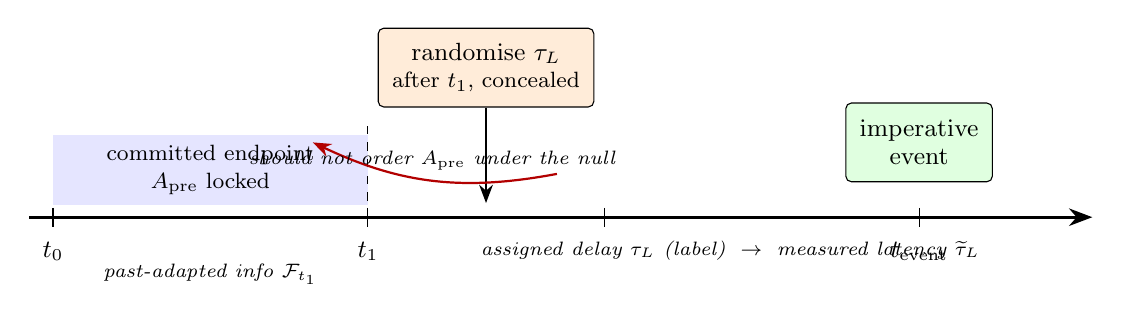
\begin{tikzpicture}[>=Stealth,font=\small,
  box/.style={draw,rounded corners=2pt,inner sep=5pt,align=center,minimum height=1.0cm},
  lab/.style={font=\scriptsize\itshape}]
% timeline
\draw[very thick,->] (-0.3,0) -- (13.2,0);
\foreach \x/\t in {0/$t_0$, 4/$t_1$, 7.0/{}, 11/$t_{\mathrm{event}}$}{
  \draw (\x,0.12) -- (\x,-0.12); \node[below=2pt] at (\x,-0.12) {\t};}
% pre-event window
\begin{scope}[on background layer]
\fill[blue!10] (0,0.15) rectangle (4,1.05);
\end{scope}
\node[align=center] at (2,0.6) {\footnotesize committed endpoint\\[-1pt]\footnotesize $\Apre$ locked};
\node[lab,below=10pt] at (2,-0.12) {past-adapted info $\F_{t_1}$};
% randomisation
\node[box,fill=orange!15] (rand) at (5.5,1.9)
  {randomise $\tauL$\\[-1pt]\footnotesize after $t_1$, concealed};
\draw[->,thick] (rand.south) -- (5.5,0.18);
\draw[dashed] (4,0) -- (4,1.25);
% delivery
\node[box,fill=green!12] at (11,0.95) {imperative\\[-1pt]event};
% arrow showing exclusion
\draw[->,thick,red!70!black] (6.4,0.55) to[bend left=18]
  node[above,lab,black]{should not order $\Apre$ under the null} (3.3,0.95);
\node[lab] at (8.6,-0.42) {assigned delay $\tauL$ (label) $\;\to\;$ measured latency $\widetilde{\tau}_L$};
\end{tikzpicture}
\caption{Post-endpoint randomisation boundary. The single-trial endpoint
\(\Apre\) is committed and locked over \(I_{\mathrm{pre}}=[t_0,t_1]\) using only
past-adapted information \(\F_{t_1}\). The trial-specific delay \(\tauL\) is
randomised only after \(t_1\) and concealed before it.
Under \textup{(R1)}--\textup{(R2)}, the assigned delay \(\tauL\) cannot order the
committed endpoint \(\Apre\) at the design stage; under \textup{(R3)}, this
exclusion is carried into the retained confirmatory analysis
(\Cref{prop:exclusion}). The measured latency \(\widetilde{\tau}_L\) is used for
auditing; the primary analysis is indexed by the assigned label \(\tauL\).}
\label{fig:boundary}
\end{figure}

% =====================================================================
\section{Endpoint, estimand and comparator}
\label{sec:endpoint-estimand-comparator}

This section fixes the three objects that must be locked before any delay label
is seen: the committed endpoint, the forward-only comparator, and the
participant-level estimand.

\subsection{Committed pre-event endpoint}
\label{sec:endpoint}

The endpoint \(\Apre^{(j)}\) is a prospectively locked, signed,
baseline-corrected single-trial feature from a committed pre-event window and
electrode set. The locked specification fixes the recording modality, channel or
source set, reference, baseline interval, endpoint window, temporal operation,
aggregation rule, sign convention, and trial-eligibility criteria. Confirmatory
preprocessing is strictly causal: an output at time \(t\) may depend only on
samples acquired at \(u\leq t\). Acausal variants may be reported only as
exploratory robustness analyses and cannot enter the confirmatory decision. The
endpoint need not be computed online at \(t_1\), but its construction rule,
eligibility rule, and sign convention become irrevocable at endpoint closure, and
later computation must remain blind to delay labels.

\subsection{Forward-only comparator}
\label{sec:comparator}

The forward-only comparator is the pre-specified high-capacity past-adapted
predictor whose job is to absorb known anticipatory structure, reduce residual
variance, and test robustness against a strong set of conventional explanations.
Its covariate set is broad but not magical. It may include elapsed foreperiod,
conditional hazard, scheduler and block-probability information, a CNV-like slow
potential amplitude, an arousal or vigilance proxy, motor-preparation proxies,
sequential trial history, reaction-time history, time on task, preprocessing
covariates, participant and session structure, and prospectively declared
interactions and nonlinear transforms. Every input must be measurable with
respect to pre-assignment information \(\F_{t_1}^{(j)}\). No realised-delay label,
and no deterministic transform of a delay label, may enter comparator fitting.

Let \(X_j\) denote the locked covariate vector and
\(m_0(X_j)=\mathbb{E}[\Apre^{(j)}\mid X_j]\) the comparator target. The family,
tuning rule, cross-fitting fold structure, and loss are fixed before delay
access. The comparator family may include penalised regression, gradient
boosting, random forests, or other pre-specified supervised predictors, provided
the family, tuning rule, fold structure, and loss are locked before delay access
\citep{Bishop2006,Hastie2009}. Folds respect randomisation blocks, and all
hyperparameter selection occurs inside the corresponding training data. For a
trial in fold \(k(j)\) the confirmatory residual is
\begin{equation}
\label{eq:residual}
\Apre^{\mathrm{resid},(j)}
=\Apre^{(j)}-\widehat{m}_0^{\,(-k(j))}(X_j).
\end{equation}
Held-out predictions and residuals are generated once and frozen before the
randomisation test; refitting the forward-only comparator inside the test is prohibited. Residualisation
improves precision and probes robustness. It is not the source of
identification. The delay contrast is identified by post-endpoint randomisation,
following the design-based logic of covariate-adjusted randomisation inference,
in which nuisance adjustment improves precision while the contrast is justified by
the assignment mechanism rather than by the predictive model
\citep{ZhaoDing2021,LuEtAl2025}.

\subsubsection*{Concrete covariate constructions}

To make the comparator class concrete, we give three constructions that together
absorb the dominant anticipatory signatures. The paradigm is assumed to vary the
\textit{cue-to-endpoint} foreperiod across trials, so that conventional preparation
varies trial to trial and is fully past-adapted, while the separate post-endpoint
delay \(\tauL\) is the randomised quantity targeted by the test. Each construction
below is \(\F_{t_1}^{(j)}\)-measurable, uses only the declared, participant-learned
schedule rather than the realised draw, and enters \(X_j\) directly.

First, a CNV-like slow-potential covariate. Let \(V_c^{(j)}(t)\) be a causally
low-pass-filtered fronto-central potential, baseline-corrected to the cue-locked
baseline, and let \(W_{\mathrm{cnv}}=[t_1-\Delta_{\mathrm{cnv}},t_1)\) be a
pre-endpoint window declared disjoint from the endpoint feature support. The
covariate is the ordinary-least-squares slope of the slow potential over that
window,
\begin{equation}
\label{eq:cnv-cov}
x_{\mathrm{cnv}}^{(j)}
=\frac{\sum_{t\in W_{\mathrm{cnv}}}(t-\bar t)\,
        \bigl(V_c^{(j)}(t)-\bar V_c^{(j)}\bigr)}
       {\sum_{t\in W_{\mathrm{cnv}}}(t-\bar t)^2},
\end{equation}
which captures the rate of the expectancy-related negativity that develops before
the endpoint closes \citep{Walter1964,Trillenberg2000}.

Second, a conditional-hazard covariate. Let \(G\) be the declared (learned)
cumulative distribution of the cue-to-endpoint foreperiod, \(g\) its density, and
\(e^{(j)}=t_1-t_{\mathrm{cue}}^{(j)}\) the elapsed foreperiod at endpoint closure.
The instantaneous and integrated hazard covariates are
\begin{equation}
\label{eq:hazard-cov}
\lambda^{(j)}=\frac{g\!\left(e^{(j)}\right)}{1-G\!\left(e^{(j)}\right)},
\qquad
\Lambda^{(j)}=-\log\!\left(1-G\!\left(e^{(j)}\right)\right),
\end{equation}
evaluated from the declared distribution at the elapsed foreperiod. They encode
the rising conditional probability that the event is imminent and use no realised
\(\tauL\) \citep{Niemi1981,Nobre2010,Coull2009}.

Third, a sequential foreperiod-history covariate. Preparation on trial \(j\)
depends on the previous trial's timing, the classical sequential effect
\citep{Steinborn2008}. We include the previous elapsed foreperiod and its signed
change,
\begin{equation}
\label{eq:seq-cov}
x_{\mathrm{seq}}^{(j)}=e^{(j-1)},
\qquad
\Delta e^{(j)}=e^{(j)}-e^{(j-1)},
\end{equation}
optionally with the previous-trial response or outcome. All three constructions,
their windows, filters, and any interactions are locked before delay access and
are computed by the same strictly causal, label-blind pipeline as the endpoint.
One subtlety deserves note: because the participant cannot perceive the endpoint
closure, their anticipatory state at \(t_1\) reflects the distribution of the full
cue-to-event interval, which the cue-to-endpoint hazard of \eqref{eq:hazard-cov}
only approximates. This misspecification affects only the residual variance, and
hence power, not the conditional-independence guarantee of \Cref{prop:exclusion},
which holds for any \(\F_{t_1}^{(j)}\)-measurable comparator regardless of its
accuracy. A hazard built from the full-interval distribution, obtained by
convolving the foreperiod schedule with the marginal delay law, may be added as a
locked covariate to recover precision.

\subsection{Participant-level estimand}
\label{sec:estimand}

The participant is the independent inferential unit; trials from one participant
are not independent biological replications. Within participant \(p\), trial
\(j\), and stratum \(\mathcal{R}_{pj}\), the assigned delay is centred at its
known scheduler mean and the participant slope is defined by
\begin{equation}
\label{eq:participant-slope}
\Apre^{\mathrm{resid},(pj)}
=\alpha_{\mathcal{R}_{pj}}
+\beta_{\tau,p}\!\left\{\tauL^{(pj)}
-\mathbb{E}_{P_{\mathrm{sch}}}\!\left[\tauL\mid\mathcal{R}_{pj}\right]\right\}
+\varepsilon_{pj}.
\end{equation}
The population estimand is the equal-participant average
\begin{equation}
\label{eq:population-slope}
\beta_\tau=\mathbb{E}_p\!\left[\beta_{\tau,p}\right].
\end{equation}
The coefficient \(\beta_\tau\) is a signed linear summary over the declared delay
support. It assumes no exponential shape and no extrapolation beyond that support.
Because the endpoint is committed before assignment, \(\beta_\tau\) is not a
forward-time treatment effect of delay on an earlier endpoint; it is the slope of
a negative-control exposure.
Two inferential routes are declared prospectively. The assignment-isolation route
holds the frozen endpoint array fixed under reassignment and is used only when
reset, washout, and lagged-delay diagnostics support endpoint-array invariance.
When the assigned delay on trial \(j\) may affect later endpoints through
carryover, adaptation, fatigue, or sequential history, the analysis uses the
sequential-score route in SI\,\S4, which treats each assignment as a
conditionally random draw given the observed pre-assignment history.
% =====================================================================
\section{Decision rule, audits and sensitivity analysis}
\label{sec:decision-audits-sensitivity}

The confirmatory decision combines a randomisation test, a participant-level
materiality bound, a set of audits, and a selection-sensitivity bound. The
commitments below are fixed before any delay label is analysed.

\subsection{Hypotheses, materiality and inference}
\label{sec:inference}

The predeclared directional hypotheses are
\begin{equation}
\label{eq:hypotheses}
H_0:\ \beta_\tau\geq0,
\qquad
H_1:\ \beta_\tau<0 .
\end{equation}
The one-sided sign is a substantive, pre-registered prior, not a property of
the design: we test specifically for a residual largest at the shortest
post-endpoint delays and decaying as the delay grows, the form a genuine
post-endpoint dependence would be expected to take. The design itself is
sign-symmetric. Under (R1)--(R3) and the past-adapted null the assigned delay
should show no material association of either sign, and a material association of
either sign that survives every audit is, by \Cref{prop:exclusion}, evidence that
the declared forward-only account is conditionally insufficient in the tested
regime. A surviving negative slope additionally confirms the pre-registered
prediction; a surviving positive slope is conditional insufficiency in the
unpredicted direction. The sign decides whether the directional prediction is
confirmed, not whether the result is real: that is decided by the sign-blind
audits, equally for both directions.

Let \(\beta_{\min}\geq0\) be the prospectively declared minimum material
magnitude, in the endpoint's native units per second or on a fixed label-blind
harmonised scale. The materiality criterion is
\begin{equation}
\label{eq:materiality}
\UCB\!\left(\widehat{\beta}_\tau\right)<-\beta_{\min}.
\end{equation}
Because no validated effect-size scale exists for a delay residual,
\(\beta_{\min}\) is a single-participant resolution floor rather than a
magnitude-of-importance threshold or a fixed population significance level. It is
the label-blind resolvability of one participant's slope,
\begin{equation}
\label{eq:beta-min-main}
\beta_{\min}=\kappa\,\frac{\sigma^{\mathrm{blind}}_{\mathrm{resid}}}
{\sigma_\tau\sqrt{\bar n_{\mathrm{ret}}}},
\end{equation}
with \(\sigma^{\mathrm{blind}}_{\mathrm{resid}}\) the label-blind within-participant
residual scale, \(\sigma_\tau\) the assigned-delay standard deviation over the
declared support, \(\bar n_{\mathrm{ret}}\) the retained trials per participant, and
\(\kappa\) a prospectively fixed multiple. The floor is not a fixed
\(\alpha\)-level test: the final support decision combines the randomisation test,
the participant-level upper bound, this resolution floor, the audits,
\(N_{\min}\), and the selection gate. The effective normal-equivalent stringency of
the upper-bound component depends on \(\beta_{\min}/\mathrm{se}_{\mathrm{pop}}\);
under a normal null approximation
\(\Pr\{\UCB(\widehat{\beta}_\tau)<-\beta_{\min}\}\approx
\Phi[-(\beta_{\min}/\mathrm{se}_{\mathrm{pop}}+1.645)]\), but this approximation
varies by many orders of magnitude with \(\mathrm{se}_{\mathrm{pop}}\) and is not a
declared test size. The confirmatory calibration is empirical and design-based,
using the randomisation distribution and simulation, not this approximation. The
floor tightens as the sample grows and guards against false positives, not against
small-but-resolvable effects. The unstandardised slope and its physical
interpretation are always reported so that scientific importance can be judged
directly. It is fixed by a registered formula evaluated only on label-blind
qualification data, never from the observed \(\widehat{\beta}_\tau\), an injected
synthetic effect, or an unblinded pilot.

Inference uses two procedures with distinct roles. The assignment-calibrated test
conditions on the committed endpoints, frozen residuals, and participant and
stratum structure, and asks whether the observed statistic is unusually negative
under the assignment mechanism actually used. Each replicate permutes fixed
multisets within declared blocks or redraws stochastic assignments from
\(P_{\mathrm{sch}}\); no replicate moves an assignment across participant,
session, or stratum. The one-sided randomisation \(p\)-value is the probability of
a statistic at least as negative as observed, with a finite-sample plus-one
correction under Monte Carlo enumeration \citep{Harris2023}. The
participant-level upper confidence bound \(\UCB(\widehat{\beta}_\tau)\) comes from
a studentised participant bootstrap-\(t\), resampling participants with all
trials and frozen residuals intact; a bias-corrected and accelerated bootstrap and
a participant \(t\)-interval are reported as sensitivity analyses. A minimum
analysable participant count \(N_{\min}\) is fixed by simulation under the planned
operating characteristics; below it, the assignment-calibrated result may be
reported but no population-materiality conclusion is drawn. Estimator details are
given in SI\,\S6.

\subsection{Decision rule}
\label{sec:decision}

A dataset receives support only when all of the following hold:
\begin{enumerate}[leftmargin=2.2em,itemsep=2pt]
\item the one-sided assignment-calibrated criterion passes;
\item \(\UCB(\widehat{\beta}_\tau)<-\beta_{\min}\);
\item the analysable participant count is at least \(N_{\min}\);
\item the randomisation, temporal-leakage, delivery, retention, and applicable
implementation-swap audits pass;
\item the prospectively calibrated selection-sensitivity bound passes
(\Cref{sec:sensitivity});
\item the prospectively declared endpoint-by-delay collider diagnostic does not
fire (\Cref{sec:sensitivity}). This is a separate requirement from the scalar
selection-sensitivity bound, which is built on the marginal retention imbalance
and cannot detect a balanced collider.
\end{enumerate}
These form one non-compensatory intersection rule; the components are not
interchangeable, and no post-result rule selects whichever procedure is more
favourable. \Cref{tab:decision} lists the resulting outcomes. Programme-level
support additionally requires independent replication using the same locked
endpoint, comparator family, materiality threshold, inference, and audit logic. A
single positive dataset supports only that dataset.

\begin{table}[t]
\centering
\caption{Estimand, null and decision outcomes for the post-endpoint
randomisation test. The estimand is the population participant-level slope
\(\beta_\tau\) of \Cref{eq:population-slope}; the null is \(\beta_\tau\geq0\).}
\label{tab:decision}
\footnotesize
\begin{tabularx}{\textwidth}{@{}p{3.5cm}p{4.3cm}X@{}}
\toprule
\textbf{Outcome} & \textbf{Statistical pattern} & \textbf{Interpretation} \\
\midrule

Supported residual &
Randomisation test rejects; \(\UCB(\widehat{\beta}_\tau)<-\beta_{\min}\);
\(N\geq N_{\min}\); audits and sensitivity bound pass. &
A materially negative assigned-delay ordering remains after the declared past-adapted analysis, conditional on the randomisation, leakage, delivery, retention, and selection-sensitivity checks. No mechanism is implied; programme-level support requires independent replication. \\
Forward-only adequate (null) &
No material negative residual; audits pass; design adequately sensitive. &
Within the declared sensitivity envelope, the forward-only account is adequate
for the tested endpoint, regime, and delay support. \\
Diagnostic failure &
Randomisation imbalance, temporal-leakage detection, preprocessing dependence,
or a failed negative control. &
The test is invalid or uninterpretable. Resolve by redesign and new data; not
evidence about sufficiency. \\
Opposite-direction departure &
Material positive slope; audits and sensitivity scrutiny applied. &
Incompatible with the pre-registered directional prediction. If it survives every
audit and the selection gate, it is conditional insufficiency of the past-adapted
account in the unpredicted direction, reported as such; it does not confirm the
prediction and requires replication. \\
Ambiguous / inconclusive &
Randomisation test and materiality bound disagree, or \(N<N_{\min}\). &
Reported descriptively; assignment-calibrated or population-materiality evidence
is insufficient for a confirmatory conclusion. \\
\bottomrule
\end{tabularx}
\end{table}

\subsection{Audits and negative controls}
\label{sec:audits}

Four audits protect the three conditions and are reported regardless of outcome.
The randomisation audit checks assignment balance across strata, seed and log
integrity, and concealment (R1). The temporal-leakage audit injects post-event
impulses and step responses into the locked pipeline and requires no committed
pre-event output beyond tolerance (R2). The delivery audit compares assigned
labels with measured latencies and bounds timing non-compliance. The retention
audit records stratum-specific delivery, rejection, missingness, and inclusion,
including the retained-against-excluded endpoint distributions available before
unblinding (R3).

Negative controls are two-sided diagnostics. A negative-control exposure or
outcome that should be unrelated to the contrast, but shows a material
association in either direction, indicates that randomisation, leakage, or
no-selection assumptions require investigation \citep{Lipsitch2010,Shi2020}. The
assigned delay is itself the primary negative-control exposure; only a materially
\textit{negative} slope is the proposed residual, while a material association of
either sign on an auxiliary negative control is a design alarm. Audit failure is
classified separately from a null: a failed audit makes the test
invalid, not evidence that the past-adapted account is sufficient.

\subsection{Omitted-pathway sensitivity analysis}
\label{sec:sensitivity}

Condition (R3) cannot be closed by inspection, so its residual risk is
quantified. The selection-sensitivity analysis reports the smallest differential,
endpoint-correlated retention or inclusion imbalance across the delay support
that could reproduce the observed slope under an otherwise past-adapted account,
and compares it with the imbalance bounded by the audits. The mapping from an
imbalance to an induced slope is computed under a declared selection-model class,
using monotone sharp bounds \citep{Lee2009} and worst-case bounds without
monotonicity \citep{Manski1990}, in the sensitivity-analysis tradition for
observational threats \citep{Rosenbaum2002}. The gate compares confidence limits,
not point estimates: support requires the lower confidence limit on the imbalance
needed to manufacture the slope to exceed the upper confidence limit on the
imbalance the audits permit. If the slope is material but this gate is not
cleared, the result is reported as selection-limited, not as support. Full
construction is given in SI\,\S8.

The scalar selection-sensitivity gate protects only against selection pathways
represented by the declared audited imbalance summary and selection-model class.
It is built on the \textit{marginal} retention imbalance across delay bins, and
marginal retention balance is not sufficient to exclude selection. A pure
endpoint-by-delay collider, in which inclusion depends on the joint configuration
of the committed endpoint and the assigned delay with no main delay effect on
retention, can manufacture a retained-sample slope while marginal retention rates
by delay bin remain approximately balanced; the full pre-selection sample still
satisfies the post-endpoint randomisation boundary, and the association arises
only after conditioning on the retained analysis sample. Because the committed
endpoint exists for every trial, this pathway is detectable directly: a
prospectively declared endpoint-by-delay diagnostic tests whether inclusion
depends on the endpoint-by-delay interaction, and the retained-against-excluded
endpoint distributions are compared within delay bins. If this diagnostic fires,
or if the retained-sample slope is compatible with an uncovered collider of the
observed magnitude under approximately balanced marginal retention, the dataset
cannot receive supported-residual classification and is reported as
selection-limited or operationally unqualified. In the benchmark this diagnostic,
not the scalar gate, is what blocks a manufactured collider slope
(\Cref{sec:benchmark-role}; SI\,\S8--\S9).

% =====================================================================
\section{Synthetic validation and practical implementation}
\label{sec:synthetic-validation}

\subsection{What the synthetic benchmarks establish}
\label{sec:benchmark-role}

The benchmarks are the pre-registered qualification of the analysis pipeline,
and their realised operating characteristics are reported in SI~\S9 and were
produced by the public benchmark package (\Cref{sec:data-access}).
They do not provide evidence that a
delay residual exists in human EEG. Before any delay labels are analysed, the
locked pipeline is run on simulated data with known generating processes, and is
required to behave as designed across seven scenarios. Under a pure forward-only
data-generating process, the delay slope must be null after the comparator: the
randomisation test should reject at its nominal rate and the materiality bound
should not clear \(-\beta_{\min}\). Under an endpoint-level injected residual, the
pipeline must recover the negative sign and approximate magnitude with the planned
estimators and sample sizes. Under an injected leakage or retention artefact, the
audits must detect it. Under a standard selection model the sensitivity bound must
move as the marginal imbalance is varied, and under a pure endpoint-by-delay
collider the dataset must be classified selection-limited rather than supported.
Under an adversarial forward-only null with nonlinear hazard structure,
heavy-tailed participant heterogeneity, heteroskedastic and autocorrelated
residuals, carryover, and comparator misspecification, false-support control must
hold. Under an opposite-direction injection the result must be classified as an
opposite-direction departure. A pipeline that fails any of these is reported as
operationally unqualified rather than as evidence for or against the sufficiency
claim.

In the realised run (run hash \texttt{0a775ac4f1ead9d3}, \(M=1000\) datasets per
scenario), the forward-only anchor produced support in \(0/1000\) datasets with the
randomisation test rejecting at \(0.050\); the adversarial forward-only null also
produced \(0/1000\) support. The endpoint-level injected residual of
\(-60\,\mu\mathrm{V\,s^{-1}}\) was supported in \(92.8\%\) of datasets. The leakage
artefact fired the temporal-leakage audit in all datasets and was never supported.
The standard selection artefact fired the retention audit in all datasets and was
never supported. The pure endpoint-by-delay collider, calibrated to approximately
balanced marginal retention, manufactured a material retained-sample slope that the
scalar selection gate passed in \(98\%\) of datasets, yet the endpoint-by-delay diagnostic
fired in all datasets, so it was classified selection-limited in \(97.9\%\) and
supported in \(0\%\). The opposite-direction injection was classified as an
opposite-direction departure in \(95.3\%\) and never as directional support. Full
realised operating characteristics, including the collider scope sweep, are
tabulated in SI~\S9.

\begin{figure}[t]
\centering

\includegraphics[width=\textwidth]{figures/CRI_synthetic_validation.pdf}
\caption{Synthetic validation of the Level~II-A decision pipeline using
simulated data, not human EEG. Anchor grid \(T_0=20\,\mathrm{ms}\) with five
assigned-delay bins \(\{0,5,10,15,20\}\,\mathrm{ms}\), \(24\) participants, and
residual noise scale \(1\,\mu\mathrm{V}\). Within each scenario the displayed
dataset is the Monte Carlo replicate whose \(\widehat{\beta}_\tau\) is closest to
the scenario median among replicates with the modal final decision. Faint lines
are participant-level bin means, filled markers are grand bin means \(\pm\)SE, and
the red line is the fitted population slope. Annotations report
\(\widehat{\beta}_\tau\), the one-sided upper bound \(\UCB\), the resolution floor
\(\beta_{\min}\) for the scenario, and the scenario support rate. Operating rates
summarise \(M=1000\) simulated datasets per generator (run hash
\texttt{0a775ac4f1ead9d3}). (a) Under a forward-only generator the residual carries
no assigned-delay slope; false support is obtained in \(0/1000\) datasets, with the
randomisation test rejecting at its nominal \(5\%\) rate. (b) With an endpoint-level
injected slope of \(-60\,\mu\mathrm{V\,s^{-1}}\) added to the committed endpoint
before comparator fitting, the pipeline recovers the negative residual and supports
it in \(92.8\%\) of datasets. (c) A post-\(t_1\) temporal leak manufactures an
apparent slope that clears the materiality floor, but the temporal-leakage audit
exceeds tolerance and fires in all \(1000\) datasets, so the non-compensatory rule
blocks support. Selection artefacts, including a balanced endpoint-by-delay
collider, are handled separately by the selection-sensitivity gate and the
endpoint-by-delay diagnostic (SI\,\S8--\S9).}
\label{fig:synthetic}
\end{figure}

\subsection{Synthetic anchor and planning power}
\label{sec:benchmark-anchor}

The reference benchmark uses a deliberately short synthetic support
\(T_0=20\,\mathrm{ms}\) with five assigned-delay bins
\(\{0,5,10,15,20\}\,\mathrm{ms}\) and, where a residual is injected, an additive
slope at the endpoint-generating level. This grid is not proposed as the empirical
horizon for anticipatory EEG. It is a low-leverage stress test of the estimator:
ordinary long-foreperiod structure is kept small, and any recovered slope must come
from the injected residual or from a deliberately injected artefact.

The injected residual is added to the committed endpoint before comparator fitting
and residualisation, not to the post-comparator residual. When the past-adapted
covariates are independent of the assigned delay by construction and the comparator
is label-blind, endpoint-level and residual-scale injection are close in the clean
anchor. The endpoint-level benchmark is nevertheless the confirmatory benchmark
because it exercises the comparator, cross-fitting, freezing, residualisation,
randomisation test, bootstrap bound, and decision rule as a single coupled
pipeline.

In the retained-sample synthetic benchmark, the estimator reaches the planning
target only when the injected slope is large relative to the residual noise and
the retained bins are balanced. The favourable grid reaches the target with
about five retained trials per bin, whereas the higher-noise grid requires about
twenty retained trials per bin. These values are synthetic estimator operating
characteristics, not EEG sample-size recommendations. An empirical protocol must
translate them into a participant-by-trial design using label-blind estimates of
residual variance, participant heterogeneity, retained-trial yield, artefact
loss, timing error, delivery compliance, and the declared materiality threshold.

The admissible delay support is itself a design variable with opposing effects:
a wider support increases assigned-delay variance and statistical leverage, but
also lengthens the interval over which ordinary foreperiod and hazard structure
operate, enlarging the burden on the comparator. The support is fixed in a
label-blind qualification sample at the point that balances leverage against the
forward-accessible structure the comparator must absorb, and is not revised
using delay information. Benchmark specifications and the planning grid are
given in SI\,\S9.

\subsection{Practical implementation sequence}
\label{sec:implementation}

The most economical programme is staged. First, qualify the hardware, scheduler,
endpoint, concealment, delivery logging, retention rules, and analysis
implementation using synthetic signals, hardware loopback data, and an
independent non-confirmatory pilot. Second, convert the design into a
full empirical protocol, preferably for
Stage~1 Registered Report review, fixing the endpoint, scheduler, comparator,
materiality threshold, sample-size rule, exclusions, audits,
selection-sensitivity analysis, and decision rule at the level required for
prospective execution. Third, run the dataset-level
test and report the audit and feasibility record regardless of outcome. Fourth,
repeat the same locked test in an independent sample. This sequence minimises
analytic flexibility and makes a surprising result expensive to fake and easy to
falsify. \Cref{fig:pipeline} summarises the analysis flow and the leakage
barriers that separate label-blind locking from confirmatory inference.

\begin{figure}[t]
\centering
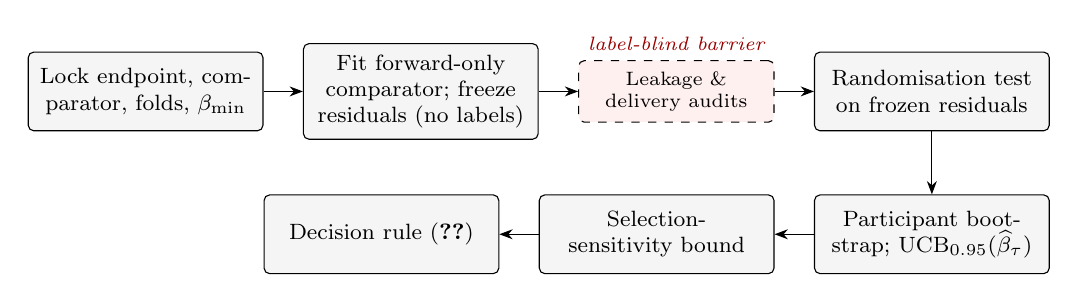
\begin{tikzpicture}[>=Stealth,font=\footnotesize,node distance=5mm,
  stage/.style={draw,rounded corners=2pt,fill=gray!8,align=center,
                text width=2.7cm,minimum height=1.0cm,inner sep=4pt},
  barrier/.style={draw,dashed,rounded corners=2pt,fill=red!6,align=center,
                text width=2.2cm,inner sep=4pt,font=\scriptsize}]
\node[stage] (lock) {Lock endpoint, comparator, folds, $\beta_{\min}$};
\node[stage,right=of lock] (fit) {Fit forward-only comparator; freeze residuals (no labels)};
\node[barrier,right=of fit] (b1) {Leakage \& delivery audits};
\node[stage,right=of b1] (rand) {Randomisation test on frozen residuals};
\node[stage,below=8mm of rand] (boot) {Participant bootstrap; $\UCB(\widehat\beta_\tau)$};
\node[stage,left=of boot] (sens) {Selection-sensitivity bound};
\node[stage,left=of sens] (dec) {Decision rule (\Cref{tab:decision})};
\draw[->] (lock) -- (fit);
\draw[->] (fit) -- (b1);
\draw[->] (b1) -- (rand);
\draw[->] (rand) -- (boot);
\draw[->] (boot) -- (sens);
\draw[->] (sens) -- (dec);
\node[above=0pt of b1,font=\scriptsize\itshape,text=red!60!black] {label-blind barrier};
\end{tikzpicture}
\caption{Analysis pipeline and leakage barriers. Endpoint, comparator, folds, and
materiality threshold are locked, and the forward-only comparator residuals are frozen, before any
delay label is accessed. Leakage and delivery audits guard the barrier between
label-blind construction and confirmatory inference. The randomisation test,
participant bootstrap, and selection-sensitivity bound feed the non-compensatory
decision rule.}
\label{fig:pipeline}
\end{figure}

% =====================================================================
\section{Discussion}
\label{sec:discussion}

This article describes a design that converts a standing assumption of
anticipatory neuroscience into a testable boundary. The assumption is that
past-adapted, forward-only processes exhaust the systematic part of pre-event
EEG. The boundary is a timing choice: commit the endpoint, then randomise the
delay. Under proper randomisation, leakage-safe preprocessing, and an adequate
forward-only comparator, the committed endpoint is conditionally independent of
the realised-delay label (\Cref{prop:exclusion}). The estimand, materiality
threshold, decision rule, audits, and sensitivity analysis make the test
falsifiable in advance and interpretable after the fact.

The warranted conclusions are deliberately narrow. A valid, adequately sensitive
null supports the forward-only account within the
declared sensitivity envelope for the tested endpoint, regime, and delay support; it
does not prove any forward model universally sufficient. A supported residual
establishes conditional insufficiency of the declared past-adapted class in that
regime, or a failure of a design assumption that the audits did not catch. It
does not, by itself, identify a cause. The first obligation following a supported
residual is to attack it: to search for failures of randomisation, concealment,
temporal integrity, delivery, retention, and inclusion, and to require
independent replication and implementation swaps.

The design generalises beyond EEG to any setting in which an outcome-relevant
variable can be assigned only after a committed measurement window has closed. In
a closed-loop brain--computer interface, for example, a control parameter applied
after a decoding window closes plays the role of the assigned delay and the
committed decoder output plays the role of the endpoint; the same boundary then
asks whether the declared past-accessible information is sufficient for that
output. The construction transfers wherever assignment, delivery, retention,
preprocessing, and inclusion can be audited with comparable rigour, so the
contribution is a reusable design-stage falsification test rather than a result.

\subsection{Relation to broader theoretical interpretations}
\label{sec:broader}

A supported and replicated residual would raise the question of what produces it.
Candidate interpretations range from mundane unmodelled forward pathways to more
speculative dynamical or physical accounts. All such interpretations are
downstream of, and outside, the evidential claim of this article. The present
test neither requires nor supports any particular mechanism, and it is designed
so that its empirical conclusion stands or falls independently of any later
theory. We therefore make no mechanistic claim here, and treat the construction
and evaluation of explanatory models as separate, prospectively specified work to
be undertaken only if and after a residual is established and replicated.

% =====================================================================
\section*{Data accessibility}
\label{sec:data-access}
This Perspective reports no human empirical data. All synthetic-benchmark numbers
in the main text, Figure~\ref{fig:synthetic}, and the electronic supplementary
material are produced by a public, executable benchmark package and recorded under
a run hash. The package (source code, configuration files, environment files, run
scripts, tests, generated tables, figure source data, and run metadata) is
available at \url{https://github.com/asopasakis/cri-leveliia-benchmark} and is
archived at \mbox{Zenodo} under DOI~\texttt{10.5281/zenodo.PLACEHOLDER}. The
figures and tables in this article were generated from the frozen output directory
with run hash \texttt{0a775ac4f1ead9d3} (\(M=1000\) Monte Carlo datasets per
scenario). Reviewers can reproduce the results with
\texttt{python scripts/run\_all.py -{}-all} followed by
\texttt{python scripts/verify\_outputs.py}.

\section*{Author contributions}
Both authors developed the design and inferential framework, specified the
benchmarks, and wrote the manuscript.

\section*{Conflict of interest}
The authors declare no competing interests.

\section*{Funding}
No specific funding supported this work.

% =====================================================================
\begin{thebibliography}{99}

\bibitem{Walter1964}
Walter WG, Cooper R, Aldridge VJ, McCallum WC, Winter AL. 1964 Contingent
negative variation: an electric sign of sensori-motor association and expectancy
in the human brain. \textit{Nature} \textbf{203}, 380--384.

\bibitem{Macar2004}
Macar F, Vidal F. 2004 Event-related potentials as indices of time processing:
a review. \textit{J. Psychophysiol.} \textbf{18}, 89--104.

\bibitem{Trillenberg2000}
Trillenberg P, Verleger R, Wascher E, Wauschkuhn B, Wessel K. 2000 CNV and
temporal uncertainty with `ageing' and `non-ageing' S1--S2 intervals.
\textit{Clin. Neurophysiol.} \textbf{111}, 1216--1226.

\bibitem{Niemi1981}
Niemi P, N\"a\"at\"anen R. 1981 Foreperiod and simple reaction time.
\textit{Psychol. Bull.} \textbf{89}, 133--162.

\bibitem{Los2001}
Los SA, Van den Heuvel CE. 2001 Intentional and unintentional contributions to
nonspecific preparation during reaction time foreperiods.
\textit{J. Exp. Psychol. Hum. Percept. Perform.} \textbf{27}, 370--386.

\bibitem{Nobre2010}
Nobre AC, Coull JT. 2010 \textit{Attention and Time}. Oxford, UK: Oxford
University Press.

\bibitem{Coull2009}
Coull JT. 2009 Neural substrates of mounting temporal expectation.
\textit{PLoS Biol.} \textbf{7}, e1000166.

\bibitem{Miniussi1999}
Miniussi C, Wilding EL, Coull JT, Nobre AC. 1999 Orienting attention in time.
\textit{Brain} \textbf{122}, 1507--1518.

\bibitem{Vanrullen2013}
VanRullen R. 2013 Visual attention: a rhythmic process?
\textit{Curr. Biol.} \textbf{23}, R1110--R1112.

\bibitem{Steinborn2008}
Steinborn MB, Langner R. 2008 Repetition and sequential effects in foreperiod
tasks. \textit{Acta Psychol.} \textbf{128}, 555--567.

\bibitem{Friston2010}
Friston K. 2010 The free-energy principle: a unified brain theory?
\textit{Nat. Rev. Neurosci.} \textbf{11}, 127--138.

\bibitem{Clark2013}
Clark A. 2013 Whatever next? Predictive brains, situated agents, and the future
of cognitive science. \textit{Behav. Brain Sci.} \textbf{36}, 181--204.

\bibitem{Hohwy2013}
Hohwy J. 2013 \textit{The Predictive Mind}. Oxford, UK: Oxford University Press.

\bibitem{Millidge2021}
Millidge B, Seth AK, Buckley CL. 2021 Predictive coding: a theoretical and
experimental review. \textit{arXiv}:2107.12979 [q-bio.NC].

\bibitem{FristonKiebel2009}
Friston K, Kiebel SJ. 2009 Predictive coding under the free-energy principle.
\textit{Phil. Trans. R. Soc. B} \textbf{364}, 1211--1221.

\bibitem{Bishop2006}
Bishop CM. 2006 \textit{Pattern Recognition and Machine Learning}. New York, NY:
Springer.

\bibitem{Hastie2009}
Hastie T, Tibshirani R, Friedman J. 2009 \textit{The Elements of Statistical
Learning}, 2nd edn. New York, NY: Springer.

\bibitem{ZhaoDing2021}
Zhao A, Ding P. 2021 Covariate-adjusted Fisher randomization tests for the
average treatment effect. \textit{J. Econom.} \textbf{225}, 278--294.

\bibitem{LuEtAl2025}
Lu X, Shi L, Liu H, Ding P. 2025 Conditional cross-fitting for unbiased
machine-learning-assisted covariate adjustment in randomized experiments.
\textit{arXiv}:2508.15664.

\bibitem{Harris2023}
Harris KD. 2023 Conditional randomization tests for behavioral and neural time
series. \textit{arXiv}:2311.03554.

\bibitem{Lipsitch2010}
Lipsitch M, Tchetgen Tchetgen E, Cohen T. 2010 Negative controls: a tool for
detecting confounding and bias in observational studies.
\textit{Epidemiology} \textbf{21}, 383--388.

\bibitem{Shi2020}
Shi X, Miao W, Tchetgen Tchetgen E. 2020 A selective review of negative control
methods in epidemiology. \textit{Curr. Epidemiol. Rep.} \textbf{7}, 190--202.

\bibitem{Lee2009}
Lee DS. 2009 Training, wages, and sample selection: estimating sharp bounds on
treatment effects. \textit{Rev. Econ. Stud.} \textbf{76}, 1071--1102.

\bibitem{Manski1990}
Manski CF. 1990 Nonparametric bounds on treatment effects.
\textit{Am. Econ. Rev.} \textbf{80}, 319--323.

\bibitem{Rosenbaum2002}
Rosenbaum PR. 2002 \textit{Observational Studies}, 2nd edn. New York, NY:
Springer.

\bibitem{Kekecs2023}
Kekecs Z \textit{et al.} 2023 Raising the value of research studies in
psychological science by increasing the credibility of research reports: the
Transparent Psi project. \textit{R. Soc. Open Sci.} \textbf{10}, 191375.

\bibitem{Bem2011}
Bem DJ. 2011 Feeling the future: experimental evidence for anomalous retroactive
influences on cognition and affect. \textit{J. Pers. Soc. Psychol.}
\textbf{100}, 407--425.

\bibitem{Wagenmakers2011}
Wagenmakers E-J, Wetzels R, Borsboom D, van der Maas HLJ. 2011 Why psychologists
must change the way they analyze their data: the case of psi.
\textit{J. Pers. Soc. Psychol.} \textbf{100}, 426--432.

\bibitem{Galak2012}
Galak J, LeBoeuf RA, Nelson LD, Simmons JP. 2012 Correcting the past: failures
to replicate psi. \textit{J. Pers. Soc. Psychol.} \textbf{103}, 933--948.

\bibitem{Mossbridge2012}
Mossbridge J, Tressoldi P, Utts J. 2012 Predictive physiological anticipation
preceding seemingly unpredictable stimuli: a meta-analysis.
\textit{Front. Psychol.} \textbf{3}, 390.

\bibitem{DugganTressoldi2018}
Duggan M, Tressoldi P. 2018 Predictive physiological anticipatory activity
preceding seemingly unpredictable stimuli: an update of Mossbridge et al.'s
meta-analysis. \textit{F1000Research} \textbf{7}, 407.

\end{thebibliography}

\end{document}
